%%%%%%%%%%%%%%%%%%%%%%%%%%%%%%%%%%%%%%%%%%%%%%%%%%%%%%%%%%%%%%%%%%%%%%%%%%%%%%%
\section{Test Case 2}
\label{sec:test-case2}
%%%%%%%%%%%%%%%%%%%%%%%%%%%%%%%%%%%%%%%%%%%%%%%%%%%%%%%%%%%%%%%%%%%%%%%%%%%%%%%

The second test case was designed to investigate the impact of the groupwise reaction rate errors in the context of an eigenvalue calculation for a PWR benchmark. The influence of the energy-integrated reaction rate errors on the global eigenvalue is evaluated in~\autoref{sec:case2-eigenvalue-bias}, while~\autoref{sec:case2-flux-bias} quantifies the relationship between the bias and reaction rate errors in the energy groups with large resonant capture cross sections.

%%%%%%%%%%%%%%%%%%%%%%%%%%%%%%%%%%%%%%%%%%%%%%%%%%%%%%%%%%%%%%%%%%%%%%%%%%%%%%%
\subsection{Eigenvalue Bias}
\label{sec:case2-eigenvalue-bias}

The OpenMC Monte Carlo code was used to simultaneously tally MGXS in 70 energy groups and compute reference eigenvalues for the second benchmark. The eigenvalues are presented in~\autoref{tab:keff-reference} for simulations with anisotropic scattering, as well as the case when OpenMC's ``iso-in-lab'' feature was employed. The two reference OpenMC simulations were also used to tally separate MGXS libraries to quantify the isotropic in lab scattering approximation used in OpenMOC and to isolate it from the flux separabilty approximation.

\begin{table}[h!]
  \centering
  \caption{Reference OpenMC eigenvalues for a 2D fuel pin.}
  \label{tab:keff-reference} 
  \begin{tabular}{c c}
  \toprule
  {\bf Anisotropic} &
  {\bf Isotropic in Lab} \\
  \midrule
  1.17488 $\pm$ 0.00001 & 1.17422 $\pm$ 0.00001 \\
  \bottomrule
\end{tabular}
\end{table}

The MGXS were employed by a series deterministic multi-group transport simulations to quantify the interaction between the energy and spatial approximations. The effects of energy discretization was analyzed by collapsing the 70-group MGXS library to coarser group structures used by the CASMO code. The MOC Flat Source Region (FSR) spatial discretization meshes were varied with constant-by material MGXS in each FSR to quantify the interaction between the energy and spatial approximations. In particular, 1, 4 or 16 radial rings were used to discretize both the fuel and moderator, while 8 azimuthal sectors were used to discretize the fuel, gap, clad and moderator. The MGXS were computed using tally meshes in OpenMC identical to the FSR meshes used by OpenMOC. All OpenMOC simulations used 128 azimuthal angles and 0.01 cm track spacing for the characteristic track laydown.

%The results underline the complex interactions between discretizations in energy and space which are impacted by the loss of angular information due ot the flux separability approximation. 

In the results that follow, the bias $\Delta\rho$ compares the eigenvalue $k_{eff}^{MOC}$ computed by OpenMOC to that of the reference eigenvalue $k_{eff}^{MC}$ computed by OpenMC in units of pcm:

\begin{equation}
\label{eqn:delta-rho}
\Delta\rho = \left(k_{eff}^{MOC} - k_{eff}^{MC}\right) \times 10^{5}
\end{equation}

\noindent The eigenvalue bias for the ``normal'' anisotropic and ``iso-in-lab'' simulations are presented in~\autoref{tab:keff-bias-aniso} and~\autoref{tab:keff-bias-iso-in-lab}, respectively, for varying energy group structures and FSR spatial discretizations. The results illustrate a strong interaction between the energy and spatial meshes used to solve the multi-group transport equation.

%In particular, the eigenvalue bias grows in magnitude with more energy groups and FSRs but is largely insensitive to the the elimination of the isotropic scattering approximation.

\begin{table}[h!]
  \centering
  \caption{The eigenvalue bias with anisotropic scattering.}
  \label{tab:keff-bias-aniso} 
  \begin{tabular}{c S[table-format=6.1] S[table-format=6.1] S[table-format=6.1]}
  \toprule
  & \multicolumn{3}{c}{{\bf FSR Discretization}} \\
  \midrule
  \multicolumn{1}{c}{{\bf \# Groups}} &
  {\bf 1$\times$} & {\bf 4$\times$} & {\bf 16$\times$} \\
  \midrule
1 & 67 & 63 & 92 \\
2 & 22 & -56 & -51 \\
4 & -58 & -128 & -135 \\
8 & -75 & -182 & -197 \\
16 & -73 & -190 & -207 \\
25 & -128 & -246 & -268 \\
40 & -131 & -261 & -288 \\
70 & -132 & -267 & -297 \\
  \bottomrule
\end{tabular}
\end{table}

%\begin{table}[h!]
%  \centering
%  \caption{The eigenvalue bias with transport-corrected MGXS.}
%  \label{tab:keff-bias-aniso} 
%  \begin{tabular}{c S[table-format=6.1] S[table-format=6.1] S[table-format=6.1]}
%  \toprule
%  & \multicolumn{3}{c}{{\bf FSR Discretization}} \\
%  \midrule
%  \multicolumn{1}{c}{{\bf \# Groups}} &
%  {\bf 1$\times$} & {\bf 4$\times$} & {\bf 16$\times$} \\
%  \midrule
%1 & 53 & 75 & 72 \\
%2 & 37 & 1 & 4 \\
%4 & -58 & -92 & -109 \\
%8 & -74 & -145 & -170 \\
%16 & -67 & -154 & -183 \\
%25 & -124 & -221 & -245 \\
%40 & -130 & -238 & -265 \\
%70 & -131 & -281 & -274 \\
%  \bottomrule
%\end{tabular}
%\end{table}

\begin{table}[h!]
  \centering
  \caption{The eigenvalue bias with isotropic-in-lab scattering.}
  \label{tab:keff-bias-iso-in-lab} 
  \begin{tabular}{c S[table-format=6.1] S[table-format=6.1] S[table-format=6.1]}
  \toprule
  & \multicolumn{3}{c}{{\bf FSR Discretization}} \\
  \midrule
  \multicolumn{1}{c}{{\bf \# Groups}} &
  {\bf 1$\times$} & {\bf 4$\times$} & {\bf 16$\times$} \\
  \midrule
1 & 80 & 55 & 66 \\
2 & 141 & 29 & 34 \\
4 & 27 & -43 & -57 \\
8 & 26 & -85 & -102 \\
16 & 35 & -91 & -111 \\
25 & -31 & -158 & -182 \\
40 & -38 & -174 & -202 \\
70 & -39 & -182 & -211 \\
  \bottomrule
\end{tabular}
\end{table}

In particular, the eigenvalue bias varies by up to 350 pcm between energy group structures and nearly 200 pcm between FSR discretizations. The use of isotropic in lab scattering in OpenMC reduces the magnitude of the bias by up to 100 pcm for seventy energy groups, indicating that the majority of the bias is unrelated to approximation error due to OpenMOC's isotropic in lab scattering kernel. Most importantly, the eigenvalue bias grows in magnitude and turns negative for increasingly fine energy group structures.


This analysis illustrates the counter-intuitive result that the bias between continuous energy Monte Carlo and multi-group deterministic transport may in fact increase in magnitude with more energy groups. Rather, these results illustrate that even when cross sections are collapsed using the ``true'' scalar flux from Monte Carlo, reaction rates are not necessarily preserved. As a result, a non-negligible eigenvalue bias emerges between continuous energy and multi-group transport calculations when increasingly fine energy group and spatial discretization meshes are used.

%  -with enough groups (e.g., ultra-fine), MG and MC eigenvalues should match exactly


%%%%%%%%%%%%%%%%%%%%%%%%%%%%%%%%%%%%%%%%%%%%%%%%%%%%%%%%%%%%%%%%%%%%%%%%%%%%%%%
\subsection{Multi-Group Flux Bias}
\label{sec:case2-flux-bias}

The analysis in~\autoref{sec:test-case1} demonstrated that the flux separability approximation leads to significant reaction rate errors in energy groups with large U-238 capture resonances for a simplified PWR fuel pin. This section investigates how such errors in resonance groups may produce the eigenvalue bias observed between continuous energy and multi-group transport calculations. The analysis in this section corresponds to OpenMOC simulations of the second test case benchmark model with a 16 radial ring FSR discretization mesh in both the fuel and moderator. As in~\autoref{sec:case2-eigenvalue-bias}, the MGXS were tallied by OpenMC directly on the OpenMOC flat source region mesh with isotropic in lab scattering.

The 70-group OpenMOC flux was compared to the reference OpenMC flux, and the percent relative error is illustrated in~\autoref{fig:rel-err-energy}. The error is given for the FSRs nearest and furthest from the moderator, along with the average error across all FSRs in the fuel. The U-238 capture cross section is also shown for comparison purposes. The figure reveals an error of up to 2.5\% in the innermost FSR in groups 24, 25 and 27. These energy groups contain the three largest U-238 capture resonances between 4 and 48.052 eV. The flux errors increase as the energy decreases through the resonance region, and the magnitude of the capture resonances increase. The one notable exception to this is group 26 (4 -- 9.877 eV) which does not include a U-238 capture resonance.

\begin{figure}[h!]
\centering
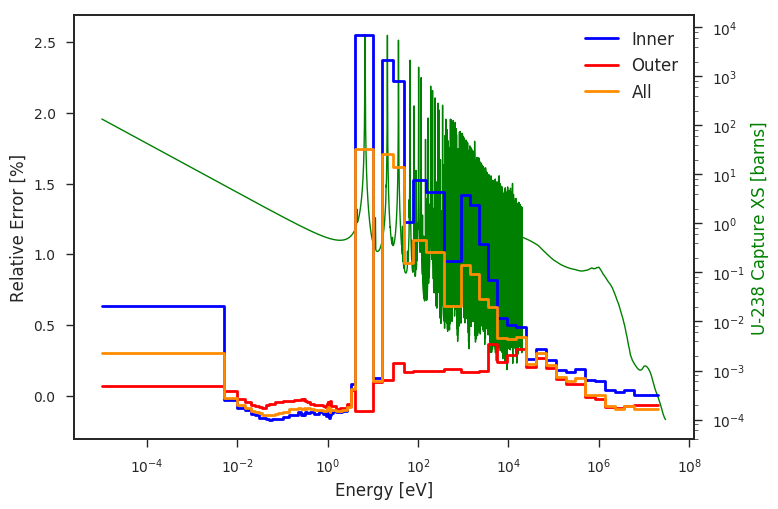
\includegraphics[width=\linewidth]{figures/rel-err-inner-outer}
\caption{The energy-dependent percent relative error of the OpenMOC scalar flux with respect to the reference OpenMC flux for the innermost, outermost and all FSRs.}
\label{fig:rel-err-energy}
\end{figure}

These observations stand in contrast to the flux errors in the outermost FSR for which no remarkable trend can be discerned. The average error across all FSRs is roughly $\nicefrac{2}{3}$ that of the innermost FSR and exhibits the same features in the resonance region. The positive error in the flux in groups with large capture resonances indicates that capture reaction rates are over-predicted in those groups by OpenMOC, contributing to the negative bias in the eigenvalue. Furthermore, these results indicate a strong relationship between the energy and spatial distribution of the flux errors.

The trends in~\autoref{fig:rel-err-energy} indicate a large difference in the error profile for those FSRs nearest and furthest from the moderator. In order to better understand this spatial variation, the flux error was analyzed in the following three energy regimes:

\begin{itemize}
  \item {\bf Range A} -- group 27 encompassing the U-238 capture resonance at 6.67 eV
  \item {\bf Range B} -- groups 11 -- 27 spanning the resonance region from 4 eV -- 408.5 keV
  \item {\bf Range C} -- groups 1 -- 70 spanning the entire energy regime from 0 -- 20 MeV
\end{itemize}

\autoref{fig:rel-err-space} highlights the spatial dependence of the error across the fuel for each energy range. The Range A error monotonically decreases from a maximum of 2.5\% to a minimum near zero in those FSRs furthest and nearest the moderator. Furthermore,  the trend accelerates in the outermost 3 -- 4 FSRs, where the error drops by nearly half of its value at the center of the pin. The error profiles for energy Range B exhibits a similar decreasing trend from the center to the rim of the pin, but the error magnitude never exceeds 0.5\% in magnitude. Finally, the Range C errors do not exhibit a marked trend and are very nearly zero for all flat source regions.

%The systematic error trends in energy and space imply that the negative eigenvalue bias is driven by a poor prediction of the reaction rates in resonance groups, as investigated in the following section.

\begin{figure}[h!]
\centering
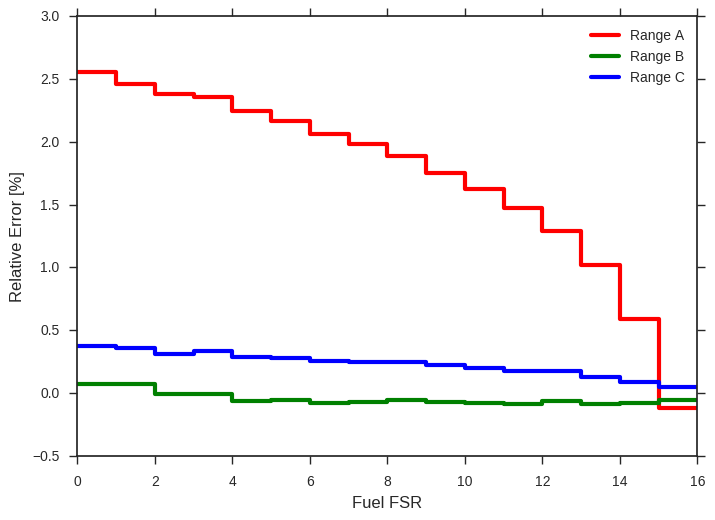
\includegraphics[width=\linewidth]{figures/rel-err-fuel-fsrs}
\caption{The spatially-varying percent relative error of the OpenMOC scalar flux with respect to the reference OpenMC flux in energy Ranges A, B, and C.}
\label{fig:rel-err-space}
\end{figure}

Finally,~\autoref{fig:u238-capture-space} illustrates the spatial dependence of the normalized U-238 capture reaction rates in Range A across the fuel FSRs. The ``rim effect'' of U-238 capture in the outermost ring nearest the moderator is illustrated by the capture rates which are are 5$\times$ greater in the outermost ring than in the innermost rings. The interior zones experience a highly self-shielded flux since neutrons at energies coinciding with the U-238 capture resonance at 6.67 eV are absorbed in the outermost ring before they can further penetrate the fuel. Although the Range A capture rates in the interior regions are relatively small, the largest errors appear in those zones as shown in~\autoref{fig:rel-err-space}. 

\begin{figure}[h!]
\centering
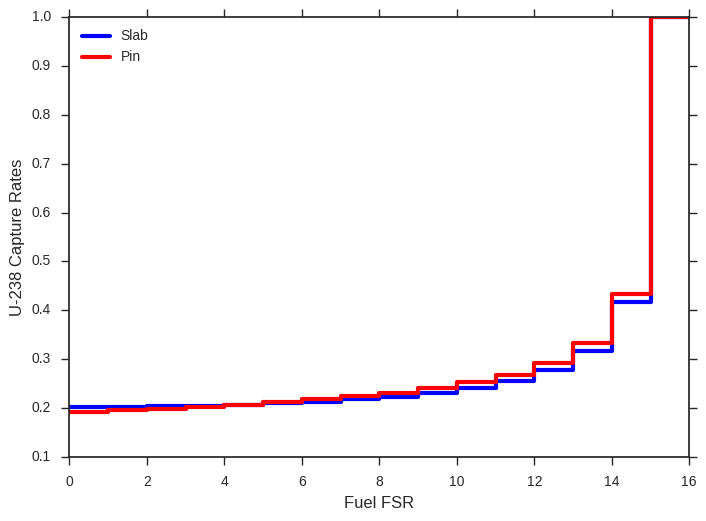
\includegraphics[width=\linewidth]{figures/u238-capt-rates-fuel-fsrs}
\caption{The normalized spatially-varying U-238 capture rates tallied by OpenMC in Range A.}
\label{fig:u238-capture-space}
\end{figure}

These results indicate that spatial self-shielding effects in resonance groups is not adequately captured by the MGXS and/or the multi-group tranport calculation. Although it is challenging to isolate the factors which convolve to bias the eigenvalue, the data presented here demonstrates that an over-prediction of U-238 capture in the resonance groups due to the flux separability approximation is the most important factor.